\documentclass[12pt,twoside]{article}
\usepackage{jmlda}

\usepackage{graphicx}
\graphicspath{ {pic/} }
\DeclareGraphicsExtensions{.pdf,.png,.jpg}
\usepackage{wrapfig}

%\NOREVIEWERNOTES
\title
    [Автоматическое построение нейросети оптимальной сложности ] % Краткое название; не нужно, если полное название влезает в~колонтитул
    {Автоматическое построение нейросети оптимальной сложности. }
\author
    {
    	Маркин~В.\,О.$^1$, 
    	Забазнов~А.\,Г.$^1$, 
    	Горян~Н.\,А.$^1$, 
    	Губанов~С.\,Е.$^1$, 
    	Таранов~С.\,К.$^1$,
    	Криницкий~К.\,Д.$^1$, 
    	Товкес~А.\,A.$^1$,
	    Улитин~А.\,Ю.$^1$
	} % основной список авторов, выводимый в оглавление
\email
    {
    	markin1198@mail.ru; 
    	antoniozabaznov@yandex.ru; goryan.na@phystech.edu; sergey.gubanov@phystech.edu; taranov.sk@phystech.edu; 
    	krinitskiy.kd@phystech.edu;
    	tovkes.aa@phystech.edu;
    	ulitin.ayu@phystech.edu
    	}
\organization
    {Московский физико-технический институт$^1$}

\abstract
{В работе рассматривается задача построения оптимальной структуры нейронной сети и исследуется вопрос устойчивости построенной модели. Для оптимизации структурных параметров используется  переход от выбора конкретной архитектуры к выбору комбинации различных архитектур сети и вариационный подход. Также исследуется влияние изменения данных на структуру сети. Для оценки качества и устойчивости моделей, построенных при помощи данного метода, проводятся эксперименты на выборке CIFAR10. Проводится сравнение предложенного алгоритма с другими методами поиска оптимальных моделей нейронной сети.

    	

\bigskip

\textbf{Ключевые слова}:  \emph{нейронные сети, автоматическое построение нейронных сетей, оптимальная структура нейронной сети}
}

\begin{document}


\maketitle


\section{Введение}
При использовании нейросетевых моделей в анализе данных часто встает вопрос о выборе архитектуры модели. Нейронная сеть имеет большое число гиперпараметров. Например, нейронная сеть, построенная по восьмислойной архитектуре AlexNet, имеет около 60 миллионов параметров. Долгое время для поиска оптимальной структуры нейросети и настройки её параметров использовались перебор и различные эвристические соображения~\cite{DBLP:conf/emnlp/Kim14}. Такие подходы вычислительно неэффективны и не дают гарантий оптимальности полученной модели.

Под оптимальной моделью понимается структура обучаемой сети и совокупность её гиперпараметров, которая даёт приемлемое качество классификации или регрессии. В данной работе в качестве критерия выбора модели предлагается сложность модели, то есть величина, учитывающая сложность описания совокупности выборки и модели. Под описанием выборки понимается приближенная оценка сложности модели, основанная на связи с её правдоподобием\cite{DescriptionLength}

Существует несколько подходов выбора модели оптимальной сложности. В работе~\cite{Cun:1990:OBD:109230.109298} представлен метод выбора модели с использованием прореживания нейронной сети, который заключается в обучении максимально большой сети, при последующем удалении части связей. Другой подход заключается в предсказании структуры модели другой нейросетью~\cite{Sutskever:2014:SSL:2969033.2969173}.

В данной работе для выбора оптимального набора гиперпараметров проводится процедура релаксации~\cite{Liu2018DARTSDA} --- переход от дискретного множества возможных значений гиперпараметров к непрерывному множетсву их комбинаций. Эта процедура позволяет параметризовать структуру модели некотором действительным вектором.
Такой подход дает возможность применять методы непрерывной оптимизации для нахождения наилучшего набора гиперпараметров. В основе разработанного метода лежит алгоритм DARTS, предложенный в работе\cite{DARTS}.
Оптимизация гиперпараметров проводится градиентными методами \cite{pmlr-v37-maclaurin15, pmlr-v70-franceschi17a, Pedregosa} либо с использованием Гауссовских процессов и Байесовской оптимизации.

Проверка и анализ метода проводится на выборке CIFAR-10\cite{CIFAR-10}. В ходе экспериментов оценивается не только качество, которое дает полученная модель но и её вычислительная сложность и устойчивость. Проводится сравнение представленного метода с эвристическими алгоритмами выбора модели, а также с алгоритмом DARTS.

\section{Постановка задачи}

Пусть заданы обучающая и вылидационная выборки:
\[
\mathfrak{D}^{\text{train}} = \{\mathbf{x}_i, y_i\}, \quad i=1,\dots,m^{\text{train}},
\]
\[
\mathfrak{D}^{\text{valid}} = \{\mathbf{x}_i, y_i\}, \quad i=1,\dots,m^{\text{valid}},
\]

состоящие из множеств пар объект-метка,
\[
\mathbf{x}_i\in\mathbf{X}\subset\mathbb{R}^{\text{n}},\quad y_i\in\mathbf{Y}\subset\mathbb{R}.
\] 

Метка $y$ объекта $\mathbf{x}$ принадлежит множеству $y\in\mathbf{Y}= \{1,\dots,Z\}$, где $Z$ - количество классов.
\\

Модель задаётся ориентированным графом $\mathbf{G=(V,E)}$, где для каждого ребра $(i,j)$ заданы базовые функции $\mathbf{g}^{i,j}, |\mathbf{g}^{i,j}| = K^{i,j}$ и их веса $\boldsymbol{\gamma}^{i,j}$. Требуется построить такую модель $\mathbf{f}$ c параметрами $\mathbf{W}\in\mathbb{R}^\text{n}$:
\[
\mathbf{f}(\mathbf{x}, \mathbf{W})= \{ \mathbf{f}_i(\mathbf{x}, \mathbf{w}_i)\}_{i=1}^\mathbf{|V|}
\]

где $\mathbf{f_i(x, w_i)}$ - подмодель c параметрами $\mathbf{w}_i$ задаётся как:
\[
\mathbf{f}_i(\mathbf{x}, \mathbf{w}_i)\ = \sum_{j\in adj(i)} \left\langle {\boldsymbol{\gamma}^{i,j}, \mathbf{g}^{i,j}} \right\rangle \mathbf{f}_j(\mathbf{x}, \mathbf{w}_j)\
\].

Тогда параметры модели определяются как конкатенация всех параметров каждой подмодели: $\mathbf{W}=[\mathbf{w}_1,\dots,\mathbf{w}_\mathbf{|V|}]$, а структура модели $\boldsymbol{\Gamma}$ задаётся вектором $\{ \boldsymbol{\gamma}^{i,j}\}_\mathbf{E}$.
\\

Функция потерь на обучении $L$ и функция потерь на валидации $Q$ задаются как:
\[
L (\mathbf{W}, \mathbf{A}, \boldsymbol{\Gamma})= \log p(\mathbf{Y}^\text{train}|\mathbf{X}^\text{train}, \mathbf{W}, \boldsymbol{\Gamma}) + \boldsymbol{e}^{\mathbf{A}}||\mathbf{W}||^2,
\]
\[
Q (\mathbf{W}, \boldsymbol{\Gamma})= \log p(\mathbf{Y}^\text{valid}|\mathbf{X}^\text{valid}, \mathbf{W}, \boldsymbol{\Gamma}) + \lambda p(\boldsymbol{\Gamma}),
\]
где $\mathbf{A}$ и $\lambda$ --- регуляризационные слагаемые, $p(\boldsymbol{\Gamma})$ - произведение всех произведение вероятностей всех $\boldsymbol{\gamma}^{i,j} \in \boldsymbol{\Gamma}$. Перед подсчётом значения  функции потерь на валидации делается априорное предположение  о распределении j том, что вектор
$\boldsymbol{\Gamma} = \{ \boldsymbol{\gamma}^{i,j}\}$ имеет распределение Дирихле\cite{Dirichlet}.
\\

Вектор $\{{\gamma}^{i,j}\}$ имеет распределение Дирихле с параметром $\alpha$, если:

\[
f(\gamma) = f(\gamma_1, \dots,\gamma_K) = 
\begin{cases}
\frac{\boldsymbol{F} (K\times\alpha)}{{\boldsymbol{F}(\alpha)}^{K}}\prod\limits_{i = 1}^K\gamma_i,\gamma \in \boldsymbol{S}
\\
0, \gamma\notin \boldsymbol{S}
\end{cases}
\]
где $\boldsymbol{F}$ - гамма-функция, $\boldsymbol{S}$ - симплекс: $\{\gamma \in \mathbb{R}^K: \sum_{i=1}^K \gamma_i = 1, \gamma_i \geqslant 0\}$.
\\

Требуется решить задачу двухуровневой оптимизации, оптимизируя параметры модели по обучающей выборке, а структуру модели по валидационной: 
\[
\mathbf{W}^*( \boldsymbol{\Gamma}) = \argmin_{\mathbf{W}}
L (\mathbf{W}, \boldsymbol{\Gamma})\]

\[
\boldsymbol{\Gamma}^*, \mathbf{A}^* = \min_{\boldsymbol{\Gamma}, \mathbf{A}} Q (\mathbf{W}^*( \boldsymbol{\Gamma}), \boldsymbol{\Gamma})
\]


\section{Релаксация}
Известно множество всех возможных операций $\mathbf{g}^{i,j} \in \mathbf{G}$. Для перехода к непрерывному пространству таких функций проводится релаксация каждой операции c использованием softmax:


$$\overline{\mathbf{g}}^{(i, j)}(x) = \sum\limits_{\mathbf{g} \in \mathbb{K}}{\frac{exp(\gamma_{\mathbf{g}}^{(i, j)})}{\sum\limits_{\overline{\mathbf{g}} \in \mathbb{K}}exp(\gamma_{\overline{\mathbf{g}}}^{(i, j)})}\mathbf{g}(x)},$$


где $\gamma^{i, j}$ --- вектор, параметризующий комбинацию базовых функций. Таким образом, путём подбора  непрерывных параметров  $\gamma$ осуществляется переход к задаче поиска базовой функции. В конце поиска, каждая комбинация базовых функций $\overline{\mathbf{g}}^{(i, j)}(x) $  меняется на $\mathbf{g}^{(i, j)} = \argmax\limits_{\mathbf{g} \in \mathbb{K}}\gamma_{\mathbf{g}}^{(i, j)}$.\\

\section{Эксперимент}

Для проверки влияния регуляризации структуры на итоговую модель был проведен вычислительный эксперимент. В качестве выборки использовалась выборка изображений CIFAR-10~\cite{CIFAR-10}. Рассматривалась задача классификации. Основным критерием качества выступал 

$$Accuracy = \frac{1}{m^\text{valid}}\sum_{\mathbf{x}, y \in \mathfrak{D}^\text{valid}} I(\mathbf{f}(\mathbf{x}), y)$$
 
 Эксперимент проводился в следующих режимах:\\
 
1) Алгоритм выбора структуры со слабой регуляризацией.\\
 В качестве регуляризации структуры выступало распределение Дирихле с параметром $\alpha = 1$.\\

2) Алгоритм выбора структуры с меняющейся регуляризацией.\\
В качестве регуляризации структуры выступало распределение Дирихле с параметром $\alpha$, меняющимся на каждой эпохи в интервале $(10^{-30}; 1)$.\\

3) Алгоритм выбора структуры с сильной регуляризацией. \\
В качестве регуляризации структуры выступало распределение Дирихле с параметром  $\alpha= 10^{-30}$.\\
 
На рис.~1 изображена общая динамика изменения структурных параметров в процессе обучения.
\begin{figure}[!htbp]
	\centering
	\subfloat[1 режим] {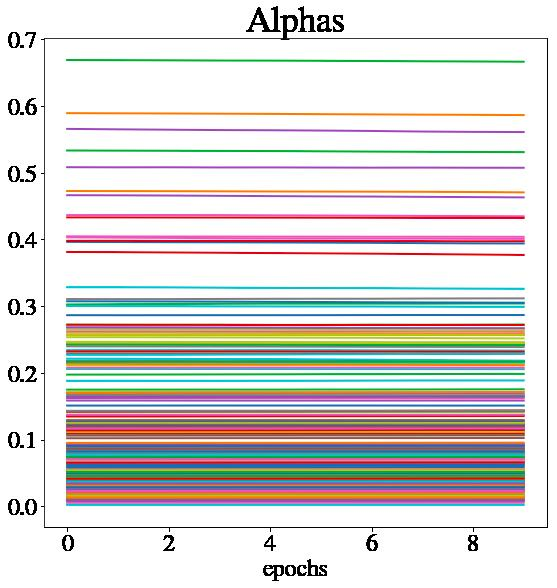
\includegraphics[width=0.5\textwidth]{pic/alphas_weak.jpeg}}
	\subfloat[2 режим] {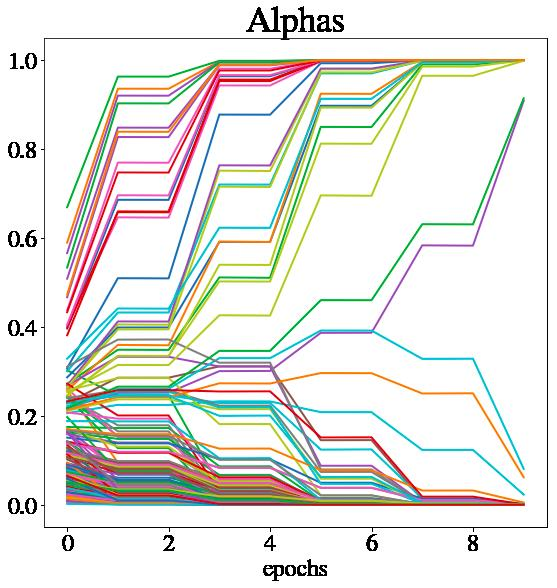
\includegraphics[width=0.5\textwidth]{pic/alphas_variable.jpeg}}\\
	\subfloat[3 режим] {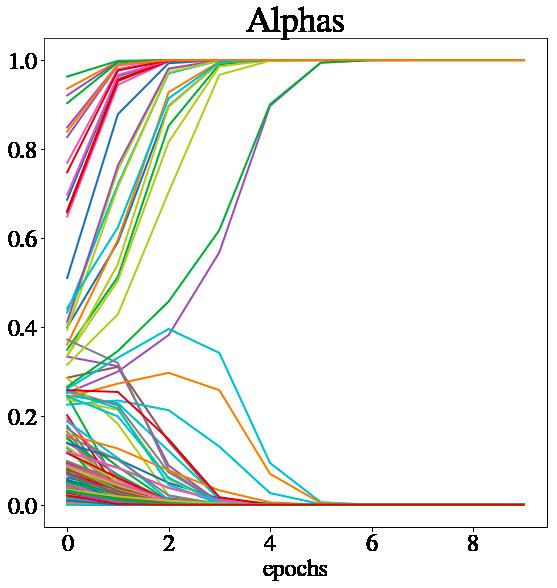
\includegraphics[width=0.5\textwidth]{pic/alphas_strong.jpeg}}
	\caption{}
	\label{}
\end{figure}

На рис.~2 для 3 запусков в каждом режиме соответствие между top-1 accuracy на тестовых данных и количеством параметров в сети, больших порога 0.1.

\begin{figure}[!htbp]
	\centering
	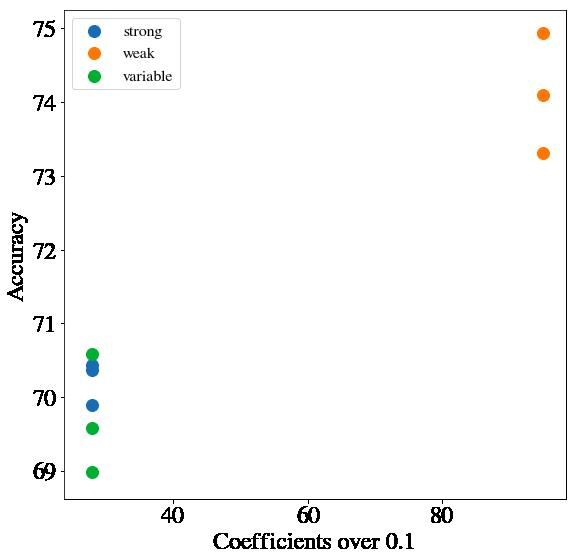
\includegraphics[width=0.5\textwidth]{pic/accuracy.jpeg}
	\caption{}
	\label{}
\end{figure}

На рис.~3 показана таблица с усредненным по 3 запускам в каждом режиме top-1 и top-5 accuracy.

\begin{figure}[!htbp]
	\centering
	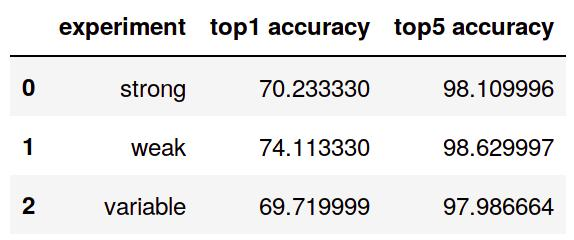
\includegraphics[width=0.5\textwidth]{pic/accuracy_table.jpeg}
	\caption{}
	\label{}
\end{figure}

Рисунок ~4 отражает поведение в сети в зависимости от присутствия в данных случайного шума, используется нормальное распределение с нулевым математическим ожиданием.
\begin{figure}[htbp]
	\centering
    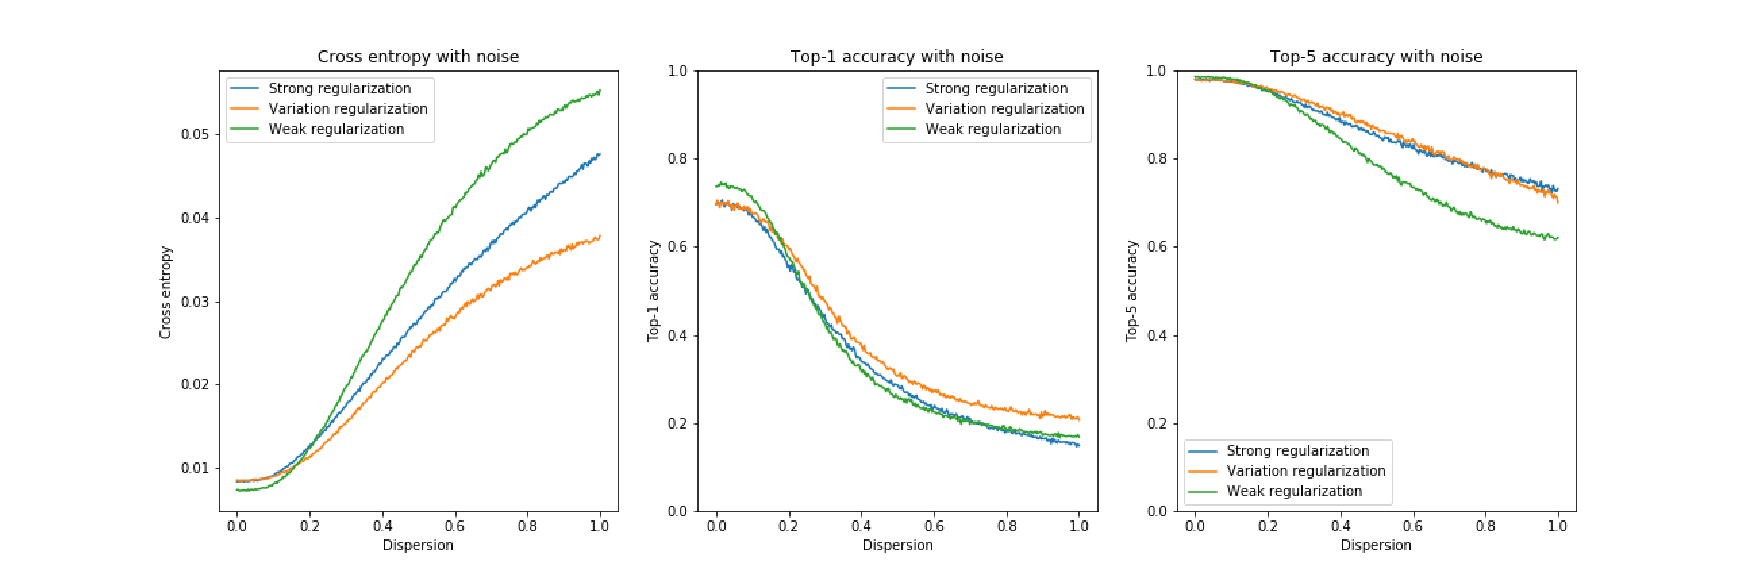
\includegraphics[width=1\linewidth]{pic/noise_graphs.pdf}
	\caption{}
	\label{}
\end{figure}

На рис.~5 также изображено поведение модели в условиях наложение случайного шума на параметры модели.
\begin{figure}[htbp]
	\centering
	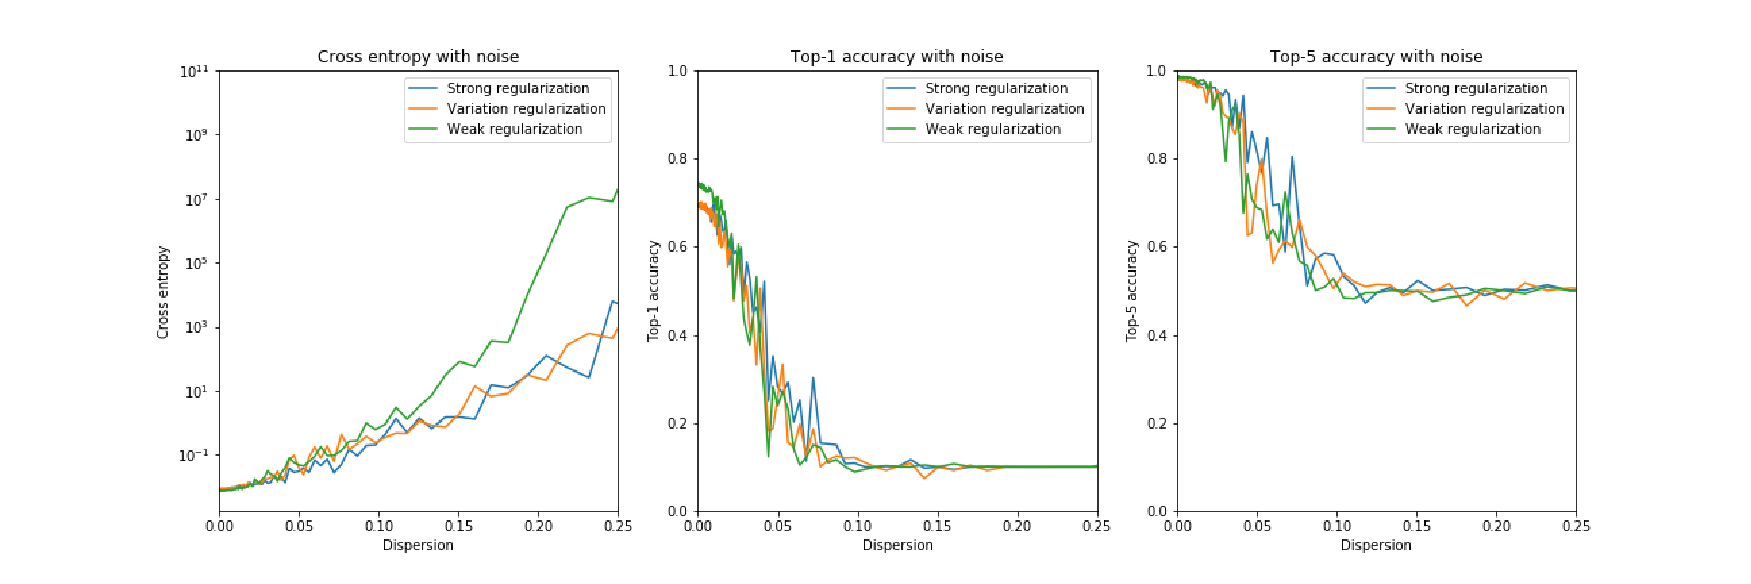
\includegraphics[width=1\linewidth]{pic/noise_params_graph.pdf}
	\caption{}
	\label{}
\end{figure}


\bibliography{report.bib}
\bibliographystyle{unsrt}

\end{document}